\documentclass[sigconf]{acmart}

\usepackage{graphicx} % For graphics
\usepackage{float} % For graphics placement, et al.
% \usepackage{amsmath} % For formulas (don't need)
% \usepackage{booktabs} % For formal tables (don't need)

\acmConference[CSPB 4502]{CU CSPB 4502 - Data Mining}{Fall 2024}{Boulder, CO, USA}
\acmYear{2024}
\acmMonth{10}

% remove ACM reference format section
\settopmatter{printacmref=false}

% remove copyright section
\renewcommand\footnotetextcopyrightpermission[1]{}

% Meta Information for the document
\title{Detecting Malicious Behaviors on Ethereum}
\author{Hallee Ray}
\affiliation{%
  \department{Computer Science Post Bacc.}
  \institution{University of Colorado - Boulder}
  \city{Boulder}
  \state{Colorado}
  \country{USA}
  \postcode{ZIP code}
}
\email{hara7620@colorado.edu}


\author{BD Tinsley}
\affiliation{%
  \department{Computer Science Post Bacc.}
  \institution{University of Colorado - Boulder}
  \city{Boulder}
  \state{Colorado}
  \country{USA}
  \postcode{ZIP code}
}
\email{beti7384@colorado.edu}

% \author{Another Author}
% \affiliation{%
%   \institution{Another Institution}
%   \city{City}
%   \state{State}
%   \country{Country}
%   \postcode{ZIP code}
% }
% \email{anotherauthor@example.com}

\begin{document}

% abstract
\begin{abstract}
The goal of our project was to elucidate a set of criteria that could potentially indicate fraudulent activity in Ethereum trading. The questions that we sought to answer included identifying trends and expected values for each of the features of the transaction data, with a speculation that outliers could indicate suspicious behavior. However, it is important to note that our dataset did not include any true labels as to whether any of the transactions were proven to be fraudulent. Therefore, all of our results are conjectured. 

We utilized K-Means to cluster and characterize the wallets. Interestingly, we identified a single wallet address across several time periods that appeared as a cluster outlier. Looking into the various features present in this cluster, we identified that this wallet was involved in far more transactions than average and executed transactions with higher than average values. Despite not being able to reliably determine if any of the transactions in the dataset were fraudulent, our data exploration and modeling helped us to generate an idea of what kind of activity we would assume to likely be fraudulent. 

Our work in this project could provide the groundwork for additional explorations into fraudulent activity and characterizing potentially risky wallets. Including additional time periods into our models could help us to further identify wallets that participate in suspicious behavior and generate a more specific set of criteria for characterizing these risky behaviors. These behavior characterizations could be used in conjunction with cryptocurrency trading applications such as CoinBase to notify individuals if the wallets they are making transactions with participate in fraudulent type behaviors. 

\end{abstract}

% keywords
\keywords{Ethereum blockchain, anomaly detection, data mining, prediction modeling, fraud detection, feature engineering, machine learning}

% main content
\maketitle

\section{Introduction}

The goal of our project was to mine data from the Ethereum blockchain to uncover trends in transactions. By analyzing historical Ethereum transaction data, we aimed to generate models that could identify if a transaction was likely fraudulent or not as well as detect fraudulent or scam-like trends that could identify investment fraud, kiosk scams, and other malicious behaviors. With the rise of cryptocurrency, there is increasing concern regarding its validity and safety. Many scams and fraudulent activity have been reported and monitored, however, due to the decentralized and unregulated nature of cryptocurrency fraud and scams are common. 

The questions that we were interested in answering about this dataset were aimed at providing us with a framework with which to identify fraudulent or suspicious activity in Ethereum transactions. Our initial goal was to answer several interesting questions related to the relationships between different features of Ethereum transactions to generate a set of criteria that would allow us to identify risky wallet behaviors. Due to the nature of our dataset, we could not ascertain with any certainty whether a transaction or wallet is fraudulent, however, we were able to identify several outliers that we suspect are likely fraudulent and understand some relative expected behaviors for wallets.

Many of our original questions that we wanted to answer included exploring correlations between the transaction features such as the time the transaction was executed and the value of the transaction. We figured that this could help us identify patterns regarding the time of day or night during which larger transactions are reported for individual wallets. Intuitively, we would suspect that fraudulent activity could occur outside of a wallet’s typical active hours, and we wanted to explore if the value of transactions outside of expected hours differ from the wallet’s usual transaction values. To address this question, we utilized several sub datasets that included all transactions within specific time periods. Due to memory restrictions, we could only reliably analyze transactions from about a month period at a time which led to the need to extrapolate these metrics from various time periods. Given these limitations, exploration into this particular question was difficult and often not meaningful due to the lack of representation and imprecise calculations.  

Another question we aimed to investigate was to find the average time between a new coin going live and its first purchase. We thought that exploring this question could provide insights into potential pump-and-dump activities. For instance, if there is a higher-than-average volume of transactions within the first 24 hours of a coin becoming available for trading, it could drive up the price of the coin, leading to a quick sell-off by investors while the price is artificially inflated. However, as our exploration of our dataset progressed, we came to realize that our dataset lacked some of this additional contextual data and we consolidated our scope to only include transactions specific to Ethereum, therefore limiting our ability to explore trends in the lifecycles of other coins. Similarly, we wished to address the average values of the transactions during the lifetime of Ethereum, and how it maps to early-stage hype. We thought that this analysis could help us recognize patterns related to a coin’s overall health in the market. Historical transaction data for Ethereum is extensive and memory restrictions of our machines prevented us from being able to generate true historical trends for the lifecycle of Ethereum to present. We did gain some interesting insights when exploring the changing transaction values for the differing time periods that we could explore, and we could gauge relative coin health by cross referencing executed transaction values with the coin’s recorded market value. 

An important question we wished to address was for coins with historical fraudulent activity, what are the general statistics for the transactions that were reported as fraudulent? The goal of this question was to generate a baseline understanding of what kinds of behavior could be flagged as potentially fraudulent. We were able to achieve more meaningful explorations into these types of metrics from our datasets, however, the dataset we utilized for this project lacked information regarding a true label of whether a transaction was valid or fraudulent. Despite this limitation, exploration into various statistical metrics for the time period of samples we pulled allowed us to identify important outliers and expected behaviors for the various features of the dataset. We were able generate plots that served to provide a visualization of where specific transactions fell in relation to the rest of the datapoints.  

We hoped that by analyzing these specific questions, we would be able to gain a deeper understanding of Ethereum transactions and improve our ability to predict whether a transaction is likely to be fraudulent. Due to the restrictions of our dataset and lack of a true label for whether the transactions were fraudulent or valid, we pivoted away from these questions. Instead, we shifted our focus to questions that would allow us to discern if a transaction was fraudulent by comparing it to general statistical expected values in conjunction with using domain knowledge.  For example, exploring statistical metrics for the values that are sent and received helped us to determine if a particular transaction was unusual due to an unusually high value. Following this idea, we generated several variables that we used as reference points for determining if a transaction was suspicious. We identified several extreme outliers that skewed the mean for many of the features, highlighted the variance in the data points, and provided guidelines for expected behaviors for the features. By plotting new transaction data against the collection of samples that we generated our variables with, allowed us to examine differences in the expected behaviors throughout different time periods of transaction data, and visualize any of the transactions could be considered unusual outliers. 

\section{Related Work}
\subsection{The Literature of Fraud Data and Identification}
Unfortunately, scams and fraudulent activity in cryptocurrency occur frequently and are difficult to monitor due to the anonymous and decentralized nature of cryptocurrency. The Federal Bureau of Investigation (FBI) and the Homeland Defense \& Security Information Analysis Center (HDIAC) have made efforts to monitor and predict fraudulent behavior in cryptocurrency.

"In February 2022, the FBI formed the Virtual Assets Unit (VAU), a specialized team dedicated to investigating cryptocurrency-related crimes" \cite{FBI2023}. In the report, the FBI identified common types of malicious behaviors using cryptocurrencies: investment fraud, recovery schemes, and kiosk scams. Investment fraud is described as malicious actors who encourage individuals to make “investments” in cryptocurrency. The FBI found that losses from cryptocurrency-related investment fraud schemes reported to the IC3 rose from \$2.57 billion in 2022 to \$3.96 billion in 2023, an increase of 53%.

Recovery schemes involve representatives from fraudulent businesses claiming to provide cryptocurrency tracing and promise an ability to recover lost funds. They request an upfront fee for this service and then immediately cease communication with the sender once the funds are received. Kiosk scams are scams where a criminal actor will direct an individual to withdraw cash from their bank and locate and send money via a kiosk or ATM-like machine. In 2023, the IC3 received more than 5,500 complaints reporting the use of cryptocurrency kiosks, with losses over \$189 million.

Knowing the existence of these scams and monitoring statistical metrics regarding cryptocurrency transactions and fraudulent activity is not sufficient to predict and prevent such scams. The Homeland Defense \& Security Information Analysis Center (HDIAC) has employed various real-time predictive machine learning models and on- and off-chain monitoring to detect fraudulent activity. The HDIAC describes the purpose of the off-chain module as preventing fraud before it occurs, whereas the on-chain module utilizes real-time surveillance to detect fraud after it has occurred \cite{HDIAC2023}.


\section{Data Set}

The dataset we used were entire blocks of transaction data on the Ethereum ledger. Our dataset incorporated block 100400 to block 1388733. In total, this dataset included nearly 2.8 million transactions. Depending on the transaction size, any given block could contain between 1 to 149 transactions, with a block containing 3 transactions on average. We were able to pull this data directly from the Ethereum ledger through a paid third party service, Infura \cite{InfuraURL}. In all, the transactions we obtained covered many days between August 17, 2015 and April 23, 2016. 

The attributes the transaction dataset contained were 
\begin{itemize}
    \item \texttt{hash}: The 64-bit unique hex identifier for the specific transaction.
    \item \texttt{nonce}: A unique, sequential integer assigned to every transaction sent from a specific Ethereum wallet address.
    \item \texttt{block\_hash}: The 64-bit unique hex identifier of the associated block.
    \item \texttt{block\_number}: The integer value of the associated block.
    \item \texttt{transaction\_index}: The integer index value of this transaction on the associated block.
    \item \texttt{from\_address}: The 64-bit unique hex identifier of the wallet account sending Ethereum.
    \item \texttt{to\_address}: The 64-bit unique hex identifier of the wallet account receiving Ethereum.
    \item \texttt{value}: The integer value of Ethereum used in the transaction.
    \item \texttt{gas}: The integer value that denotes the computational work required to execute the transaction as set by the network.
    \item \texttt{gas\_price}: The integer-valued cost per unit of computational work set by the \texttt{from\_address} in Ethereum.
    \item \texttt{input}: The hex value data payload of the transaction.
    \item \texttt{block\_timestamp}: The integer value that represents the time its associated block was created or mined.
    \item \texttt{max\_fee\_per\_gas}: A newly incorporated feature that specifies the maximum total gas price the \texttt{from\_address} is willing to spend for this transaction \citep{LondonHardfork}.
    \item \texttt{max\_priority\_fee\_per\_gas}: Another newly incorporated feature which specifies the maximum tip in Gwei (ETH $10^{-9}$) that the \texttt{from\_address} is willing to send to validators to prioritize this transaction \cite{LondonHardfork}.
    \item \texttt{transaction\_type}: An integer value to denote the type of transaction this one is, as incorporated in EIP-2718 \cite{TypedTransactions}.
    \item \texttt{max\_fee\_per\_blob\_gas}: The integer value in Gwei the \texttt{from\_address} is willing to spend to store larger “blob” type data in storage, as incorporated in EIP-4844 \cite{ProtoDanksharding}.
    \item \texttt{blob\_versioned\_hashes}: Hex-valued addresses to the data storage blobs, as incorporated in EIP-4844 \cite{ProtoDanksharding}.
\end{itemize}

Due to the daily limits imposed on the Infura billing model, we were able to pull around 130,000 transactions in a 24-hour period over the course of several days.  

\section{Main Techniques Applied}


\subsection{Data Cleaning \& Preprocessing}
For data preprocessing, we needed to clean the data of empty values. We found that, due to the timeframe of our dataset, many of the newer attributes (\texttt{max\_fee\_per\_blob\_gas}, \texttt{blob\_versioned\_hashes}, \texttt{max\_fee\_per\_gas}) were empty because those features were added to Ethereum transactions well after the transactions in our dataset. Furthermore, the default value for \texttt{transaction\_type}, \texttt{0x0}, was present for all transactions. The label \texttt{0x0} for transactions implied they were legacy transactions, which did not add helpful information for distinguishing any single transaction from others. Therefore, we removed it.

Due to the high verification standards of the data on the Ethereum blockchain, we found that no other columns contained data requiring further processing or imputation. Aside from a few small quirks, such as several transactions with a \texttt{to\_address} of \texttt{0x} followed by 40 hexadecimal zeroes, colloquially known as the \textit{genesis block}, the dataset presented a coherent story of transactions that we could attempt to analyze \cite{GenesisBlock}.

\subsection{Exploratory Data Analysis \& Feature Engineering}

Once the data was cleaned, we did a brief exploration into each of the features to ensure that there were no missing values and that the datatype of the features made sense for what was being portrayed and to extrapolate important information that we wished to use in our later modeling and anomaly detection.  

One of the goals of our project was to generate an understanding of trends in Ethereum transaction data over the lifecycle of the coin. Therefore, one of the first features we explored was the date time feature. We created additional columns in the dataset that provided more granularity for the date, including the year, month, and day, with hopes to visualize transaction fluctuations and trends across years, months, and even days. Introducing this additional granularity was not ultimately useful for the datasets that we utilized for our exploration, anomaly detection, and prediction modeling because it did not provide enough representation for the varying time periods. We were only able to pull about a month’s worth of data at a time, which prevented us from exploring trends within months and years in terms of the entire life of the coin.

Other features had interesting data types that we hoped to normalize or convert into usable values for our models. The input feature was noted to be a string data type with strings on varying lengths. These appeared to be strings of addresses or hexadecimal values that could be used to track the usage of the coin. There was huge variance in the length of these variables and with lack of domain knowledge for how to extrapolate usage indicators from these strings, we were unable to normalize these values. Similarly, we expected the value type feature to provide useful information about the usage of the transaction. Exploration into this feature identified only one transaction type for our time periods which unfortunately provided no value to our models. Due to the computational complexity of modeling with string variables, and a lack of insightful information from the transaction type, we ultimately decided to drop these features from our dataset with considerations to further explore them for future steps. 

We then explored the statistical metrics of several of the features we considered to be highly likely to indicate fraud such as transaction value and gas usage. We generated graphs of these metrics to identify any outliers and visualize the skew of the values. In addition to exploring the general trends of the entire sample, we created visualizations that highlighted particularly interesting wallets. We hoped that this exploration would illuminate the variance of these features and provide us with ways to determine behavioral characteristics of these wallets.   

Additionally, we generated and analyzed the correlation matrix of the features to identify interesting relationships between the features. Surprisingly, many of the features that we expected to be correlated with each other did not have any strong correlations. This indicated that our anomaly detection would need to consider a wider range of features to characterize potentially fraudulent behavior since no two or three features could reliably provide information about the expected trends of another. 

\begin{figure}[H]
    \centering
    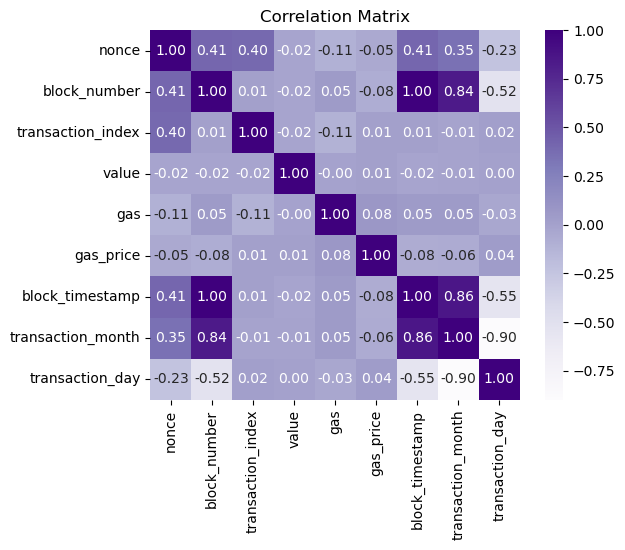
\includegraphics[width=0.8\linewidth]{M4-correlation-matrix.png}
    \caption{Correlation matrix of features showing intuitive correlations.}
    \label{fig:m4CorrelationMatrix}
\end{figure}

The main goal of our feature engineering included gaining and understanding about the behaviors of specific wallets. We included features that allowed us to characterize the wallets as senders or receivers as well as gain insights into typical transaction and gas values for the wallets. By including these features related primarily to the value of the transactions, frequency of transactions, and the gas usage for specific wallets, we aimed to provide more specific information on individual practices. The goal of this was to apply these individualized characterizations to new transaction values where we could create warnings for users about interactions with other wallets or red flag behaviors within their own wallets. To generate these statistics, it was important to filter out the values where the value sent or received was 0, as this shows the direction of the transaction; if the from value is zero, the to value is nonzero meaning this transaction was sent from the wallet. 

The features that we engineered for this dataset included to and from frequency, the total and average values that the wallets received and sent, as well as the total and average gas used in sent and received transactions, and the price of the gas for sent and received transactions. Intuitively, transactions with high gas might indicate fraud because when an individual sets a high gas fee that they are willing to pay, it ensures that the transactions are prioritized and successful. Pump and dump schemes also often lead to spikes in gas fees. When executing transactions through a centralized exchange, the exchange includes the fees and gas considerations in the transaction fee, whereas executing transactions through the Ethereum network directly allows the user to set the gas fee. It would make sense that transactions that occur over the Ethereum network directly are more likely to be fraudulent than transactions that occur through a centralized exchange. By exploring the frequency of transactions, we hoped to uncover wallets that may be involved in pump and dump type activity where they may execute many transactions that leads to price gouging and sell off the resource when the price is inflated. 

Finally, we engineered features that explored the interpersonal relationships of wallets. By identifying which wallets engaged in transactions with many other wallets, we hoped to create classifications for the type of wallet. For example, we hypothesized that wallets with a high number of distinct counterparties could represent wallets that executed transactions on behalf of a business, where the business may except Ethereum as a form of payment. We also hypothesized that wallets that executed many transactions with itself could be characterized as an investment account.  

Overall, the goal of our exploratory data analysis was to gain an understanding of the general trends and expected behaviors of Ethereum transactions, as well as to create a set of criteria that could potentially be used to classify wallets in regard to their individual transaction behaviors. 

\subsection{Anomaly Detection}
Our anomaly detection was highly reliant on comparisons between individual transactions and the expected behaviors identified by our statistical analysis and feature engineering. To explore these relationships, we decided that creating a set of reference visualizations would be useful. We compared several of our engineered features for individual wallets with the mean transaction values, gas used, and gas prices. These features were plotted against lines showing the value of the mean and the value of the upper bound for these features. The upper bounds for these metrics were calculated by adding the value of the third quartile to 1.5 times the interquartile range. Unfortunately, due to the presence of extreme outliers, the upper bound often fell below the value of the mean, however, these visualizations provided useful insights into a relative count of how many wallets fell outside of our generated expected values.  

	These visualizations could then be used to compare the change in the expected behaviors of wallets over time. For example, trends that we have seen in cryptocurrencies is an increase in value over time. Our reference images were generated with data from the early life of Ethereum. Intuitively, we expected the average value of transactions in ETH for the entire dataset and individual wallets to decrease for data from later time periods. For example, the average price of Ethereum between 8/17/2015 and 9/13/2015 was between 0.87 and 1.35 USD and the average price of Ethereum between 8/17/2024 and 9/13/2024 was 2,223.93 and 2,769.10 USD. If a wallet’s average transaction value from 2015 was 100ETH, or about \$87 - \$135, we would expect the average transaction value of the same wallet in 2024 to be about 0.04ETH, ignoring potential changes in personal finances, inflation, etc. 

\begin{figure}[H]
    \centering
    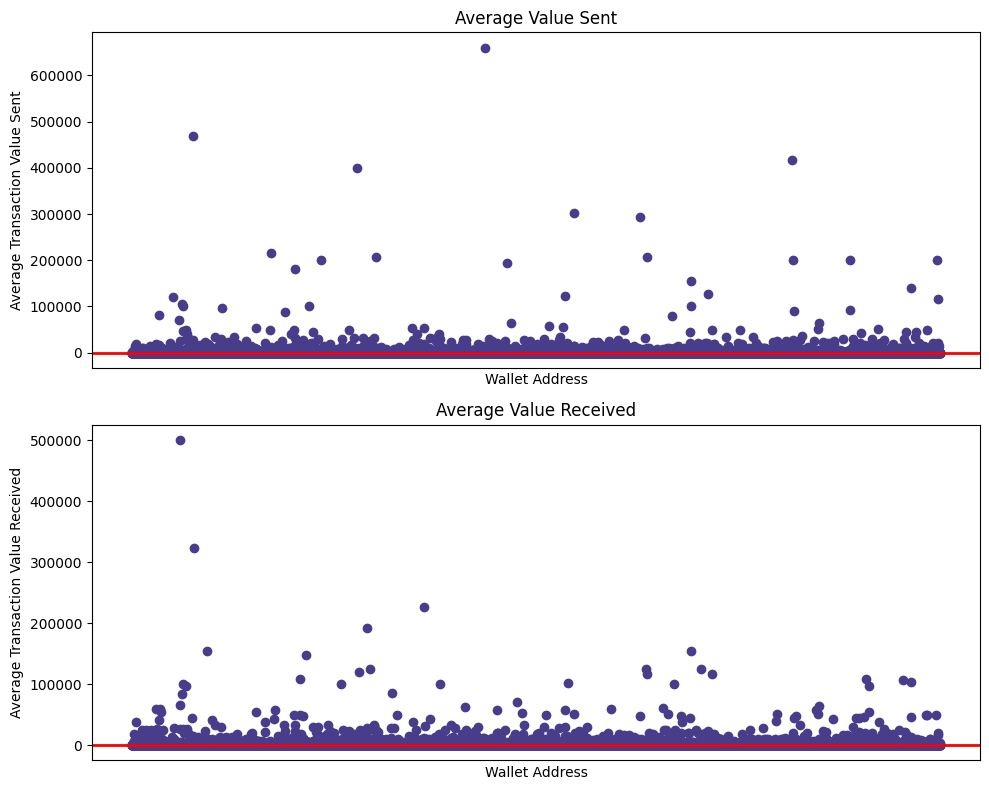
\includegraphics[width=0.8\linewidth]{M6-2-avg-val.png}
    \caption{Scatter plots of average values sent and received.}
    \label{fig:m6StackedAvgVal}
\end{figure}

The average gas that is used in transactions could also be used to help in characterizing types of transactions. Gas fees are determined by the resources needed in order to execute the type of transaction. For example, transferring Ethereum between two wallets is considered a basic transaction and typical fees are 21,000 gas units to complete the transaction. Looking at the typical gas used for transactions for each wallet could help us to identify what kinds of transactions each wallet often participates in and classify typical wallet behavior. This information could be used to flag whether a transaction is typical for a specific wallet.

\begin{figure}[H]
    \centering
    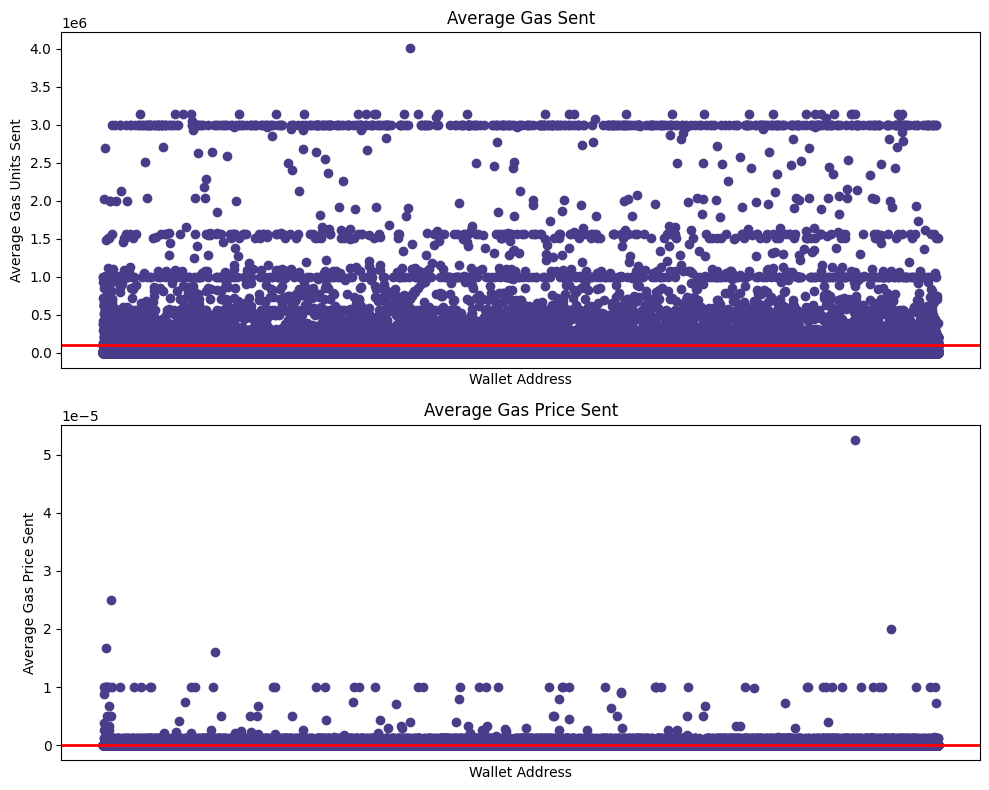
\includegraphics[width=0.8\linewidth]{M6-2-avg-gas-sent.png}
    \caption{Scatter plots of average gas sent.}
    \label{fig:m6StackedAvgGasSent}
\end{figure}
	

\subsection{Prediction Modeling}
We wished to expand on our anomaly detection by creating prediction models to generate an idea of whether a transaction is potentially fraudulent. We utilized K-Means to generate clusters based on our prior engineered features that give us insights into wallet behaviors. To visualize the separation of the clusters created by our trained K-Means models, we utilized PCA to reduce the dimensions to 2 and generate a scatter plot of the datapoints in the clusters.  

Due to the nature of our problem in identifying transactions as fraudulent or not, we wanted to first consider a K-Means model with only 2 clusters with the hopes that it would accurately delineate between ‘likely fraudulent’ and ‘likely not fraudulent’. To get an idea of the relative accuracy and quality of the clusters for this model, we utilized the silhouette score. The silhouette score for our model with two clusters was very high, indicating that the clusters were well defined and separated from each other. We analyzed the values of the centroids for each feature to gain insights into the meanings of each cluster.  

\begin{figure}[H]
    \centering
    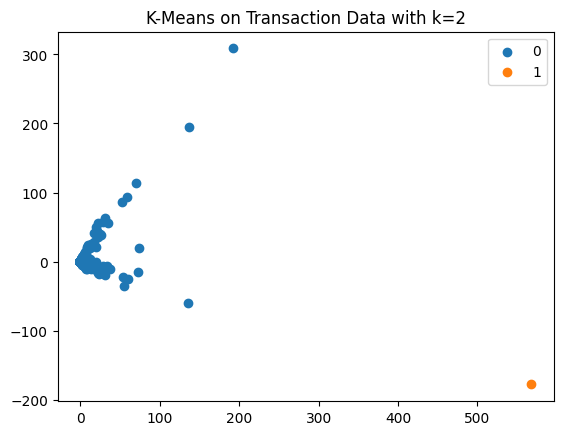
\includegraphics[width=0.8\linewidth]{M6-k-2.png}
    \caption{K-Means with 2 clusters.}
    \label{fig:k2Clusters}
\end{figure}

To optimize our model and generate the highest silhouette score, we followed the elbow method and generated a graph of the inertia of various K-Means models with different numbers of clusters. The inertia of the K-Means model is a measure of the distance between each data point and the cluster centroid, indicating how well the dataset is clustered. Following this elbow method, we identified that the lowest inertia, therefore best clustering, occurred in K-Means models with 5 to 8 clusters. We were curious about the separation of these model’s clusters, so we generated visualizations for models with 5, 6 and 8 clusters.

\begin{figure}[H]
    \centering
    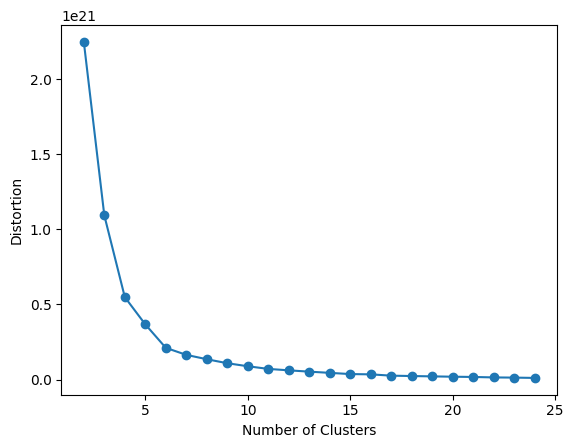
\includegraphics[width=0.8\linewidth]{M6-elbow.png}
    \caption{Hypertuning with the 'elbow method'.}
    \label{fig:ElbowMethod}
\end{figure}

Following this elbow method, we identified that the lowest inertia, therefore best clustering, occurred in K-Means models with 5 to 8 clusters. We were curious about the separation of these model’s clusters, so we generated visualizations for models with 5, 6 and 8 clusters. These models all had high silhouette scores that we used to understand the relative accuracy of the models. In analyzing these models, we hoped to understand general differences between the behaviors for transactions in each of these clusters. Exploring the centroids of each cluster helped us to reason about characteristics of the wallets in each cluster. Additionally, we looked into the specific wallets that were clustered into what we deemed outlier clusters so that we could analyze wallet specific values for transaction frequency, gas usage, and transaction values.  

\begin{figure}[H]
    \centering
    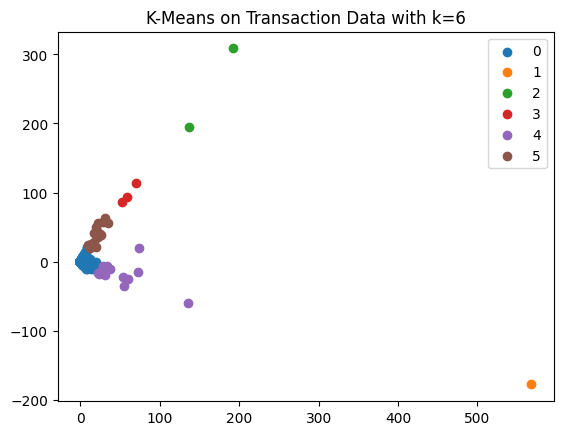
\includegraphics[width=0.8\linewidth]{M6-k-6.png}
    \caption{K-Means with 6 clusters.}
    \label{fig:k6Clusters}
\end{figure}

\section{Key Results}

This process allowed us to discover general trends in Ethereum transactions for each of the time points we considered. To understand characteristics and behaviors of the data points, we utilized K-Means clustering. When analyzing the best hyperparameters for optimizing our clustering model, we performed the elbow method to reveal the optimal number of clusters for our dataset. Initially, we thought that two clusters would be sufficient such that we could delineate between likely fraudulent and likely not fraudulent. However, the elbow method indicated that the optimal number of clusters was between 5 to 8. To visualize the separation of these clusters, we performed dimensionality reduction with PCA and then plotted the generated labels. To analyze the relative quality of the clusters in each of our models with different numbers of clusters, we utilized the silhouette score. This score is used to determine the quality of the clusters in terms of their separation and how well each data point is clustered. All our models had very high silhouette scores, indicating that the models successfully characterized the activity of the data points in each cluster. By considering the centroid values for each feature in each cluster, we could generate a criterion of defining behaviors for each cluster. For example, our model with two clusters appeared to separate the data into wallets that executed a huge number of sending transactions for small values, whereas the other cluster had comparable numbers of sent and received transactions for higher values. 

The results of our clustering identified one key wallet that appeared as an outlier across several different time ranges. This wallet in particular had an extremely high number of transactions that it received. This wallet received the most transactions of any of the wallets with an average value received that was greater than the third quartile, indicating an unusual number of transactions for the time period. Additionally, despite sending fewer transactions, the values that this wallet sent far exceeded the third quartile.  The average gas used for this wallet was also higher than the population mean. Intuitively, these findings allowed us to characterize the behavior of this wallet. The high gas could indicate that the wallet wanted to prioritize these transactions in the block chain, which could point to potentially fraudulent activity due to increased pressures for transaction success. The huge number of transactions that this wallet received could indicate that the wallet processes transactions on behalf of a business. Additionally, the transactions this wallet received had higher than average values, which could support the idea that this could possibly belong to a business or a successful scam wallet. Analyzing this wallet in terms of distinct counterparties indicated that this wallet executed transactions with the highest number of other wallets. These findings highlighted interesting behaviors that we considered to be likely fraudulent. We could then consider these characteristics when analyzing feature values of other wallets. 

While we were unable to determine with any certainty whether any transactions were fraudulent, we did gain valuable insights into expected behaviors for wallets. We also considered the time frame for each dataset that we used and referenced historical data in order to conceptualize the values of transactions in US dollars. When we were generating statistical metrics for the dataset, we discovered that the max average value that a single wallet sent was 935800.0ETH. The price of ETH during between 8/17/2015-9/13/2015 was between 0.87 and 1.35USD, therefore, 935800.0ETH during this time was 814,146 - 1,263,330 USD \cite{EthHistorical}. This wallet could have only one sent transaction that was the cause of this average, however, this is an outlier. Additionally, 75\% of the data had average sent values of 126.652167ETH or less. This value far exceeds the interquartile range and upper boundary, and likely would be considered as a red flag for suspicious behavior.  

Other interesting discoveries that we made during our exploration included the identification of several wallets with interesting wallet addresses that could potentially represent "placeholder" or testing wallets. The first of these wallets only received transactions, with the average value of each transaction it received being about 2 ETH or somewhere between about 1.74 to 2.70 USD. The other two wallet addresses processed fewer transactions with even smaller amounts, supporting the idea that these wallets could represent testing wallets. During our exploratory data analysis, we uncovered that the outliers we detected skewed the data so far that the majority of the data for many of our engineered features fell way below the mean. 


\section{Applications}
The knowledge that we gained during our data exploration and modeling provided us with insights with which we could apply to other datasets and time periods to hypothesize whether any transactions are likely fraudulent. With additional information regarding known fraudulent activity, we could extend our modeling to include supervised models that could classify a transaction as fraudulent or not, instead of describing the transaction in terms of activity and behavior. 

Future applications of the knowledge gained in this project includes generating a flagging system for users who trade Ethereum. Utilizing the behaviors and typical behaviors for wallets, we could generate a warning message for users who are about to engage in activity with wallets that are outside of the expected behavior of historical transactions as well as activity types for the specific wallet. 




\bibliographystyle{ACM-Reference-Format}
\bibliography{references} 

\end{document}